\begin{frame}{Generators}
    
\begin{itemize}
    \item A generator $G$ is a network that maps a simple distribution (for example, a normal distribution) $\pi(z)$ to a complex data distribution $p_G(x)$, which aims to be as close as possible to the real data distribution $p_{\text{data}}(x)$.
\end{itemize}
\begin{figure}
    \centering
    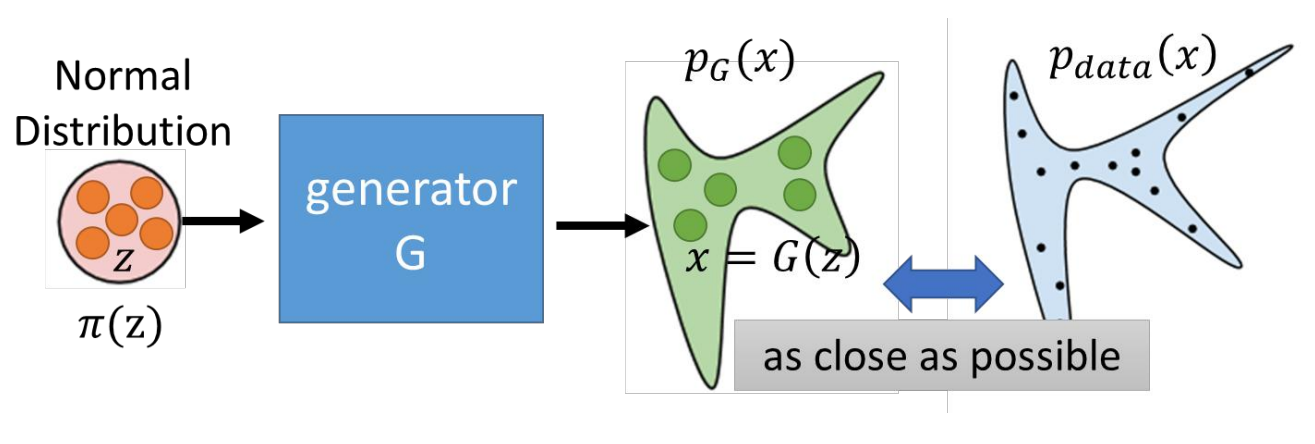
\includegraphics[height=0.5\textheight, width=\textwidth, keepaspectratio]{images/norm-flow/nfm_gen.png}
    \caption*{The goal of a generator network in a generative model}
\end{figure}
\end{frame}
